\documentclass[a4paper,12pt,reqno]{amsart}
\usepackage{macros_M66}

\graphicspath{ {images/} }

\begin{document}
%%%%%%%%%%%%%%%%%%%%%%%%%%%%%%%%%%%%%%%%%%%%%%%%%
\hautdepage{TP2: Interpolation par morceaux et splines}
%%%%%%%%%%%%%%%%%%%%%%%%%%%%%%%%%%%%%%%%%%%%%%%%%

Vous êtes invités à créer le fichier \cmd{tp2\_fonction.sci} qui sera complété au fur et à mesure avec les nouvelles procédures. Pour chaque exercices il va falloir créer un fichier, \cmd{tp2\_exo0.sce}, \dots ,\cmd{tp3\_exo1.sce}, comportant les lignes de code correspondant à la résolution de l'exercice et incluant au début le fichier \cmd{tp2\_fonction.sci} et les autres initialisations habituelles (\mtlb{clear},\mtlb{clc},\dots).\\[1ex]

\attention{center}{En cas de blocage, commencez toujours par regarder l'aide ou sur Google !!}


% ==================================
\section{Présentation et indications}
% ==================================

On se propose ici de procéder à l'interpolation d'une fonction $f$ définie sur un intervalle $I=[a,b]$ par utilisation de fonctions polynomiales par morceaux. On découpe donc l'intervalle en $n$ sous-intervalles de même longueur $h=(b-a)/n$ définis par $I_i=[x_{i-1},x_{i}[$, avec $x_i=a+ih$, $1 \leq i \leq n$. Sur chaque $I_i$, on approchera $f$ par un polynôme $\pi_{i}$ de degré fixé (ce degré va varier selon les exercices).

\begin{center}
  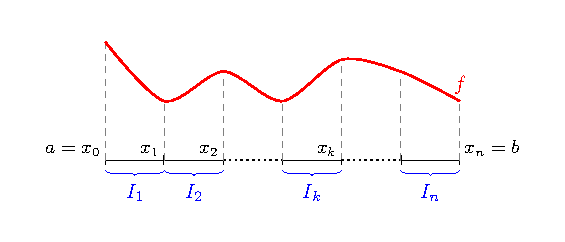
\includegraphics[width=15cm]{FonctionParMorceaux}
\end{center}


% ==================================
\section{Exercices}
% ==================================

\setcounter{numeroexo}{-1} % on commence par l'exo 0
% --------------------------------------------
\begin{exo} (Détermination de l'intervalle)

  Avant de procéder aux différents interpolations, on va créer une fonction utilitaire. Cette fonction nous permetera étant donné un $x \in [a,b[$ de déterminer le sous intervalle d'apartenance.

\begin{center}
  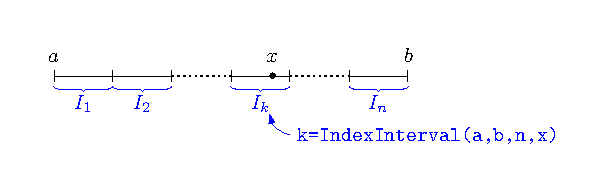
\includegraphics[width=15cm]{IndexInterval}
\end{center}

  Pour cela, créez dans le fichier \cmd{tp2\_fonction.sci} une fonction \mtlb{[k]=IndexInterval(a,b,n,x)}. Cette fonction doit satisfaire les contisions suivantes:
  \begin{itemize}
    \item Étant donnés les bornes \mtlb{a} et \mtlb{b}, le nombre de sous intervalles \mtlb{n} et un vecteur \mtlb{x}, elle doit retourner un vecteur \mtlb{k}, de la même taille que \mtlb{x}, qui contient les indices des intervalles contenant les coordonées de \mtlb{x}.

    \item Pour des raisons téchniques, on demande en plus que si une coordonné de \mtlb{x} est inférieur à \mtlb{a}, la valeur corréspondante rendu doit être \mtlb{1}, et si elle est supérieur où egale à \mtlb{b}, elle doit être \mtlb{n}.
  \end{itemize}

  \textit{Indications:}
  \begin{enumerate}
    \item Avant de débuter la création de la fonction, testez et commentez le code suivant
    \begin{matlab}
      test = [-1.3 -0.5 0.7 1.3 2 3.7];
      disp(ceil(test));
      disp(max(test,1));
      disp(min(test,2));
    \end{matlab}

    \item Créez d'abord la fonction pour qu'elle fonctionne avec une valeur unique \mtlb{x}. Puis testez la par exemple avec avec \mtlb{IndexInterval(0,1,3,.5)} (le résultat doit être \mtlb{2}).

    \item Une fois la fonction faite pour fonctionner avec un vecteur \mtlb{x}, vérifier que l'instruction \mtlb{IndexInterval(0,1,3,[-1,0,.5,1,2])} renvoie \mtlb{1.    1.    2.    3.    3.}.
  \end{enumerate}

\end{exo}


% --------------------------------------------
\begin{exo} (Interpolation constante par morceaux)

  Dons cette exercice on va approcher une fonction $f$ par une fonction constante par morceaux.
  \begin{enumerate}
    \item Une fonction constante par morceaux sur $n$ sous-inervalles de $I=[a,b]$ de longueur constante, peut être encodé par un vecteur $v=(v_{1},\ldots,v_{n})$ :
    \begin{center}
      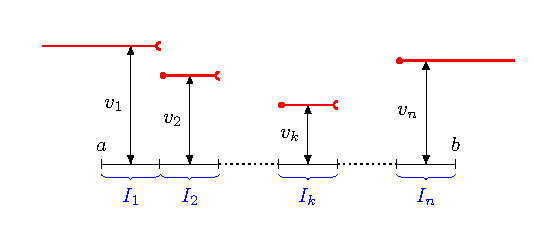
\includegraphics[width=10cm]{ConstParMorceaux}
    \end{center}
    Créez la fonction \mtlb{[y] = ConstPiecewise(a,b,v,x)} qui étant données les bornes \mtlb{a}, \mtlb{b} et les valeurs des hauteurs des paliers \mtlb{v}, renvoie les valeurs \mtlb{y} de la fonction constante par morceaux aux points \mtlb{x}.\\
    Puis pour tester son fonctionnement, dessinez (en utilisant $1000$ points) la fonction affine par morceaux sur $[-\frac12, \frac32]$ qui a pour hauteur des paliers $v=(0,2,-1,1)$. Profitez de l'occasion pour rajouter, en plus de la légende, une grille \mtlb{xgrid(5, 1, 7)} visible sur la boite de coordonnés \mtlb{axes.data_bounds = [-1,2,-2,3]}, où \mtlb{axes=gca()}. Le résultat devrait rassemble à ça :
    \begin{center}
      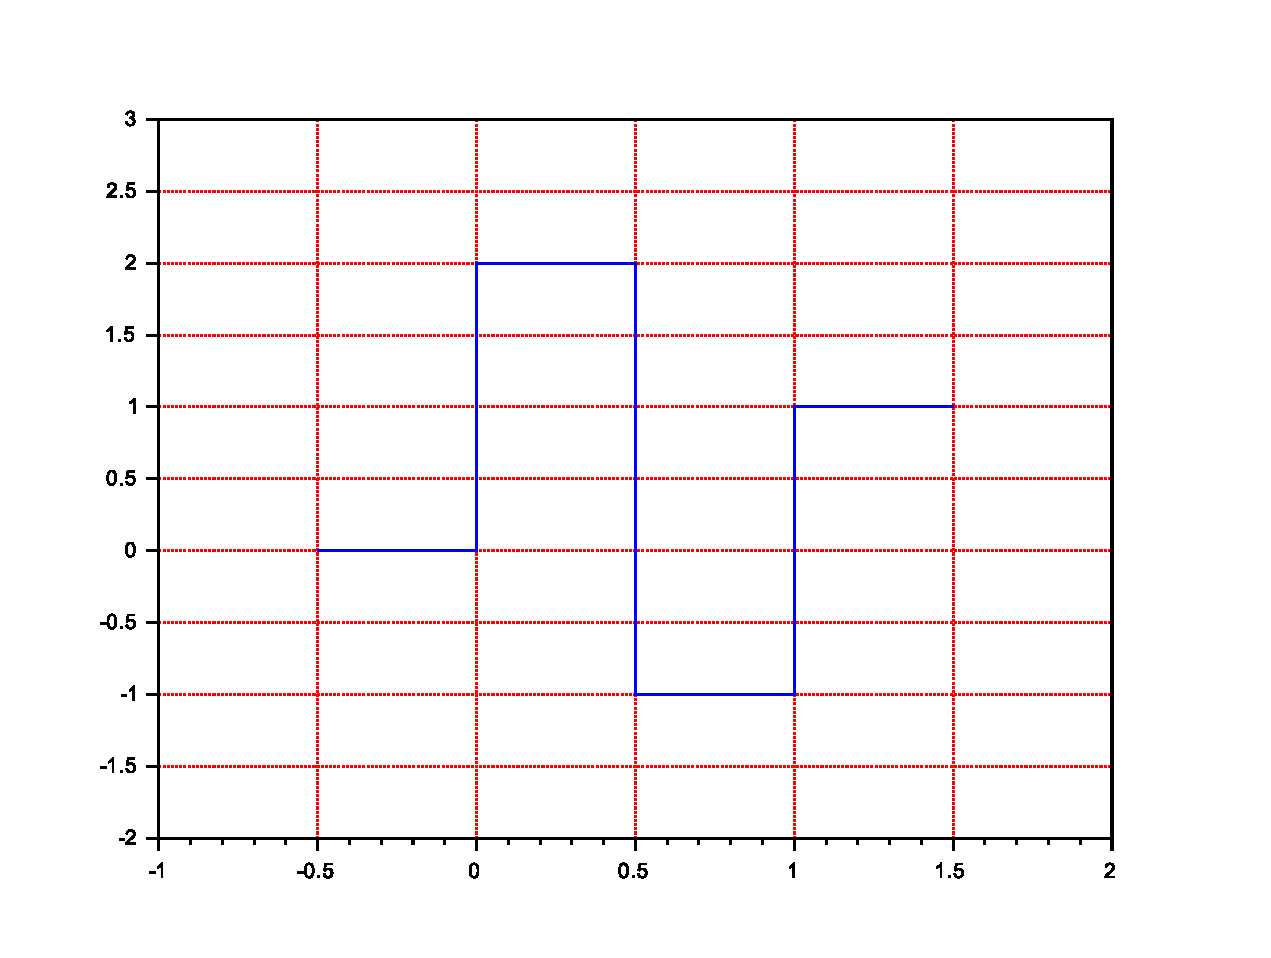
\includegraphics[width=11cm]{SciLab_test_constante}
    \end{center}

    \item On se propose maintenant de construire une fonction $s_0$ constante sur chaque intervalle $I_i$ telle que $s_{0|_{I_i}}(x)=f(x_{i-\frac12})$, où $x_{i-\frac12}=(x_{i-1}+x_{i})/2$. En supposant que  $f \in C^1(I)$, on rappelle que :
      \[
        ||f-s_0||_{\infty}\leq \frac{h}{2} M_1,
      \]
    où $M_1$ est un majorant de $f'$ sur $I$.
    \begin{enumerate}
      \item Pour cela, créez une fonction \mtlb{[v,t] = InterpConst(a,b,n,f)} qui étant donné une fonction \mtlb{f} renvoie dans \mtlb{t} les valeur des $x_{i-\frac12}$ pour $i=1,\ldots,n$, et en \mtlb{v} les valeurs de $f$ en ces points.

      \item Soit $f=\sin(x)$ sur $[-5,5]$. En utilisant les fonctions précédemment définies, \mtlb{InterpConst} et \mtlb{ConstPiecewise}, dessinez (en utilisant 1000 points) sur un même graphique:
      \begin{itemize}
        \item la fonction $f$,
        \item la fonction d'interpolation constante par morceaux $s_{0}$,
        \item les points d'interpolation $(x_{i-\frac12},f(x_{i-\frac12}))$.
      \end{itemize}
      Le résultat devrait rassemble à ça :
      \begin{center}
        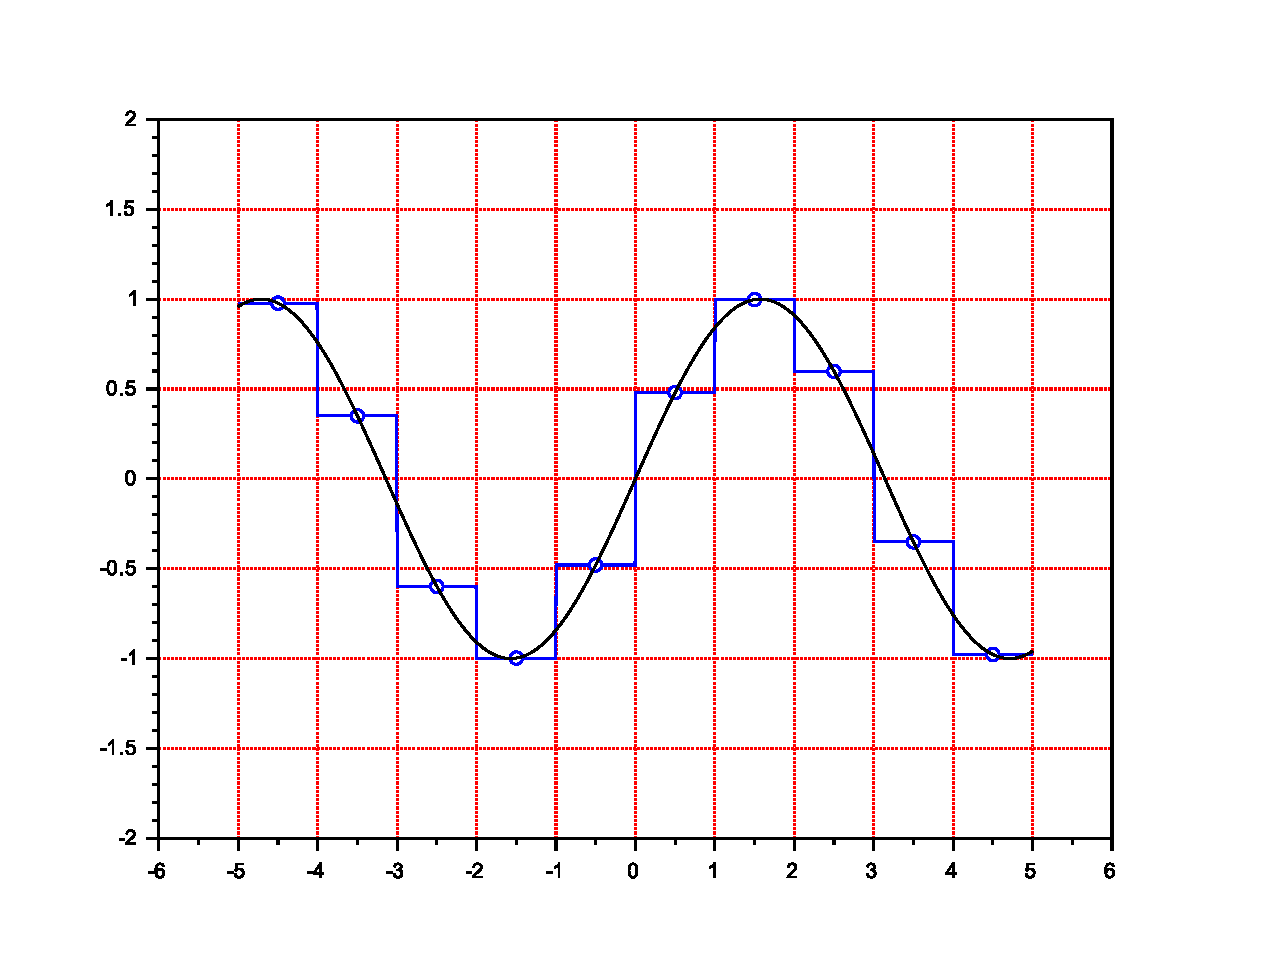
\includegraphics[width=11cm]{SciLab_test_interp_constante}
      \end{center}

      \item Pour \mtlb{n=10:100} calculez l'erreur d'interpolation (en norme infinie). Puis sur un même graphique représentez (en échelle logarithmique) cette erreur et la majoration théorique de l'erreur.
    \end{enumerate}
  \end{enumerate}
\end{exo}


% --------------------------------------------
\begin{exo} (Interpolation affine par morceaux)

  Dons cette exercice on va approcher une fonction $f$ par une fonction affine par morceaux.
  \begin{enumerate}
    \item Une fonction affine par morceaux sur $n$ sous-inervalles de $I=[a,b]$ de longueur constante, peut être encodé par un vecteur $v=(v_{1},\ldots,v_{n+1})$:
    \begin{center}
      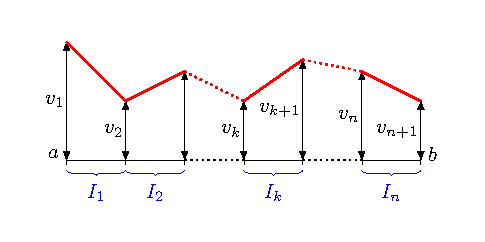
\includegraphics[width=11cm]{AffineParMorceaux.pdf}
    \end{center}
    Créez la fonction \mtlb{[y] = AffinePiecewise(a,b,v,x)} qui étant données les bornes \mtlb{a}, \mtlb{b} et les valeurs aux nœuds \mtlb{v}, renvoie les valeurs \mtlb{y} de la fonction affine par morceaux aux points \mtlb{x}.\\
    Puis pour tester son fonctionnement, dessinez (en utilisant $1000$ points) la fonction affine par morceaux sur $[-\frac12, \frac32]$ qui a pour valeurs aux nœuds $v=(0,2,-1,1,0)$. Le résultat devrait rassemble à ça :
    \begin{center}
      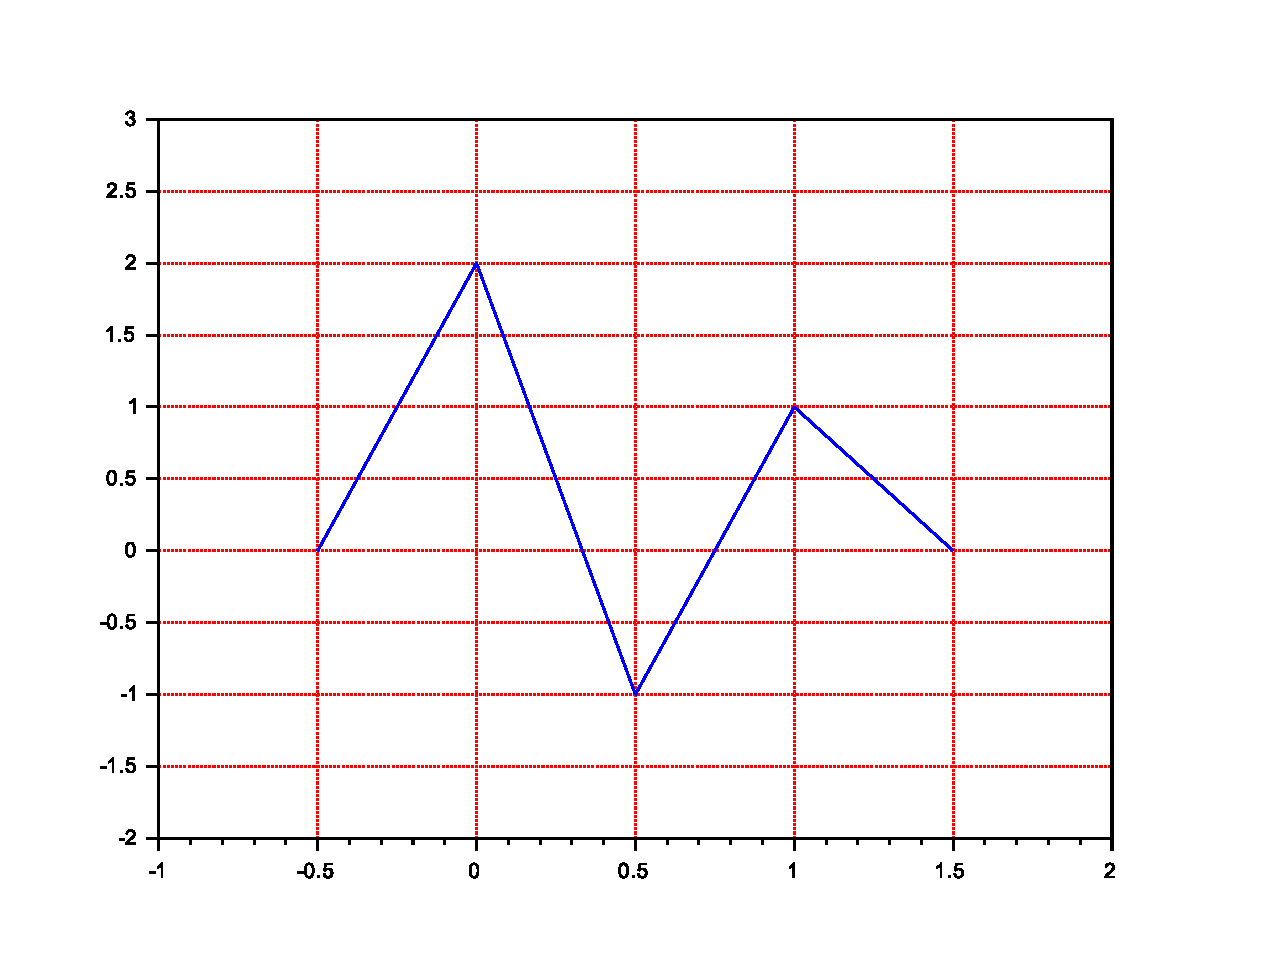
\includegraphics[width=11cm]{SciLab_test_affine}
    \end{center}

    \item On se propose maintenant de construire la fonction $s_1$ affine sur chaque intervalle $I_i$ et qui coïncide avec $f$ aux points $x_i$ et $x_{i+1}$ :
      $$
        s_{1|_{I_i}}(x)= \frac{(x_{i+1}-x)f(x_i)+(x-x_i)f(x_{i+1})}{h}.
      $$
      En supposant que $f \in C^2(I)$, on rappelle que  :
      $$
        ||f-s_1||_{\infty}\leq \frac{h^2}{8} M_2,
      $$
      où $M_2$ est un majorant de $f''$ sur $I$.\\
      On va suivre le même schéma que dans l'exercice précédent.
      \begin{enumerate}
      \item Créez une fonction \mtlb{[v,t] = InterpAffine(a,b,n,f)} qui étant donné une fonction \mtlb{f} renvoie dans \mtlb{t} les valeur des $x_{i}$ pour $i=0,\ldots,n$, et en \mtlb{v} les valeurs de $f$ en ces points.

      \item Soit $f=\sin(x)$ sur $[-5,5]$. En utilisant les fonctions précédemment définies, \mtlb{InterpAffine} et \mtlb{AffinePiecewise}, dessinez (en utilisant 1000 points) sur un même graphique:
      \begin{itemize}
        \item la fonction $f$,
        \item la fonction d'interpolation affine par morceaux $s_{1}$ sur $10$ intervalles,
        \item les points d'interpolation $(x_{i},f(x_{i}))$.
      \end{itemize}
      Le résultat devrait rassemble à ça :
      \begin{center}
        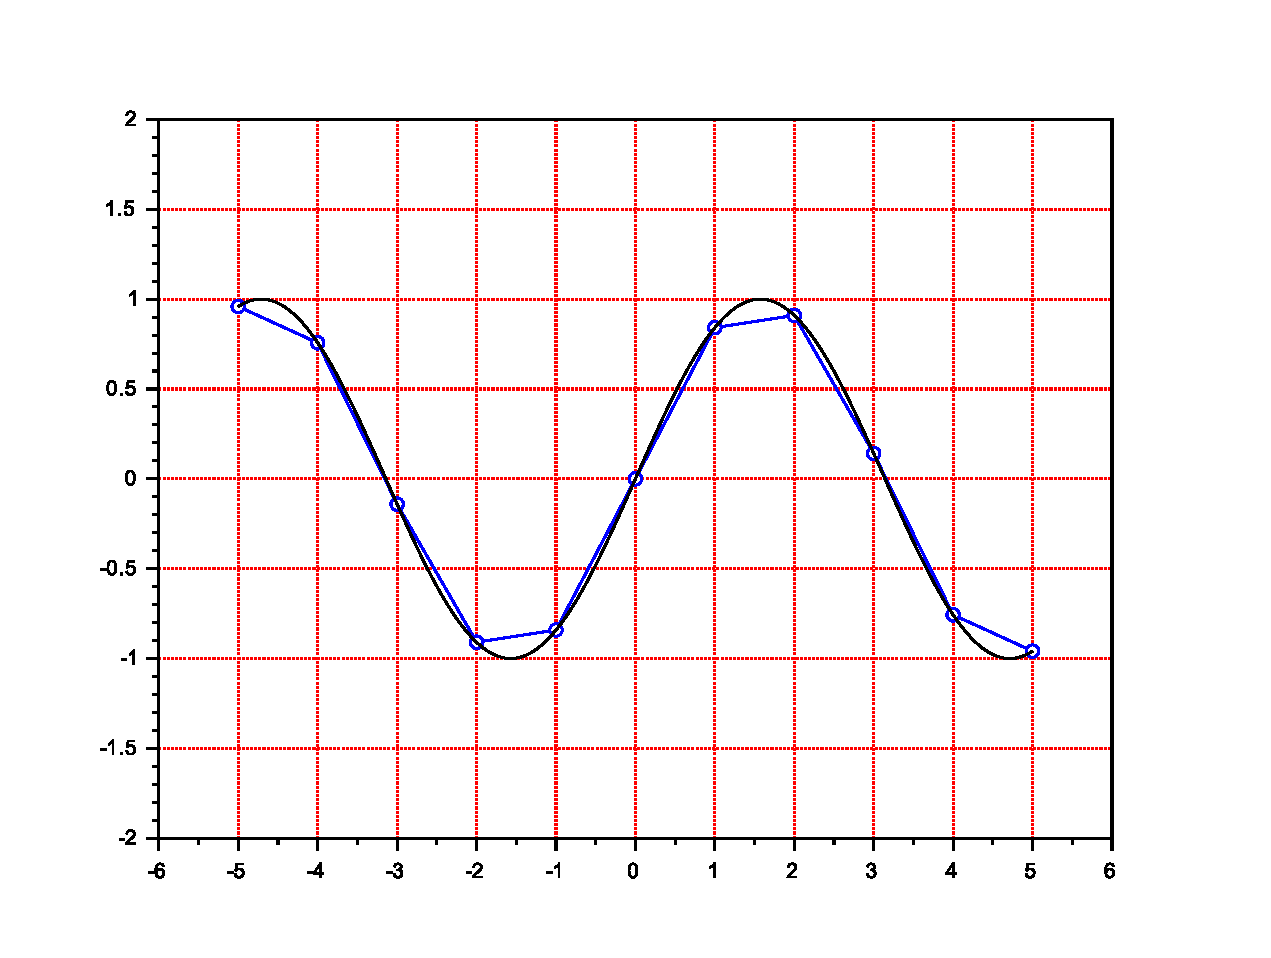
\includegraphics[width=11cm]{SciLab_test_interp_affine}
      \end{center}

      \item Pour \mtlb{n=10:100} calculez l'erreur d'interpolation (en norme infinie). Puis sur un même graphique représentez (en échelle logarithmique) cette erreur et la majoration théorique de l'erreur.
    \end{enumerate}
  \end{enumerate}
\end{exo}

% --------------------------------------------
\newpage
\begin{exo} (Interpolation par splines)

  Dons cette exercice on va approcher une fonction $f$ par une spline cubique (fonction $C^{2}$ polynomiale de degré $3$ par morceaux).
  \begin{enumerate}
    \item Dans cette question on va déterminer les coefficients d'un polynôme cubique à partir des données d'interpolation d'Heermit. Pour commencer, écrire une procédure\\
    \indent \mtlb{[p] = CubicCoeffs(x1,x2,y1,y2,d1,d2)}\\
    qui détermine les coefficients \mtlb{p} du polynôme $P(x)= p_{1}+p_{2}x+p_{3}x^{2}+p_{4}x^{3}$ qui a pour valeurs \mtlb{y1} en \mtlb{x1} et \mtlb{y2} en \mtlb{x2}. Et dont les dérivées dans ces deux points sont respectivement \mtlb{d1} et \mtlb{d2}. Pour vérifier que votre procédure fonctionne, tester la avec \mtlb{CubicCoeffs(0,1,2,3,4,5)} et le résultat devrait être \mtlb{2. 4. - 10. 7.} (éventuellement en colonne).
    \begin{center}
      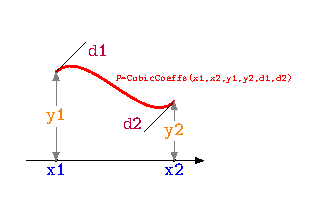
\includegraphics[width=9cm]{CubbicCoeffs}
    \end{center}

    \item Écrire la procédure \mtlb{[y] = CubicEval(p,x)} qui étant donné les coefficients \mtlb{p} d'un polynôme et un vecteur \mtlb{x}, évalue ce polynôme en les coordonnées de \mtlb{x}. Pour vérifier que votre procédure fonctionne, tester la avec \mtlb{CubicEval([1:4],[-1:1])} et le résultat devrait être \mtlb{- 2.    1.    10.}.

    \item En utilisant les procédure \mtlb{CubicCoeffs} et \mtlb{CubicEval} dessiner la base d'Hermit sur $[0,1]$, c'est-à-dire les $4$ polynômes qui ont une seul des valeurs $P(0)$, $P(1)$, $P'(0)$, $P'(1)$ non nul, égale à $1$.

    \item En utilisant les procédure \mtlb{CubicCoeffs} et \mtlb{CubicEval} dessiner les polynômes $P$ sur $[0,1]$ tels que $P(0)=0$, $P(1)=1$, $P'(1)=-7$ et $P'(0)$ prend les valeurs entières de $-10$ à $10$.

    \item Il est temps maintenant de créer la procédure qui évalue la spline cubique d'interpolation. Pour cela créer la procédure \mtlb{[y] = CubicSplinEval(a,b,v,x)} qui a pour entrées:
    \begin{itemize}
      \item Les bornes \mtlb{a} et \mtlb{b} de l'intervalle d'interpolation.

      \item Les valeur \mtlb{v=[v(1), v(2), ..., v(n)]} d'interpolation aux  $n+1$ nœuds équi-distribués.

      \item Les points \mtlb{x} dans lesquels il faut faire l'évaluation.
    \end{itemize}
    Et qui renvoie les valeurs \mtlb{y} de la spline naturelle aux points \mtlb{x}.

    \begin{center}
      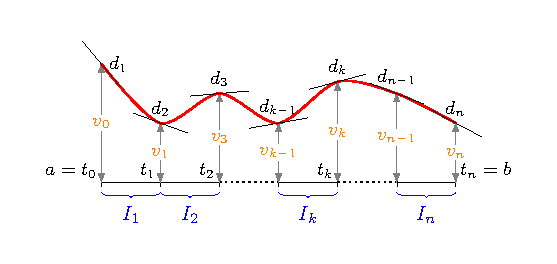
\includegraphics[width=15cm]{CubbicSpline}
    \end{center}

    Cette procédure devra faire dans l'ordre:
    \begin{itemize}
       \item Créez le vecteur \mtlb{t} des $n+1$ nœuds équi-distribués d'interpolation.
       \item En utilisant \mtlb{d = splin(t,v,"natural")}, déterminez les valeurs dés dérivées aux nœuds d'interpolation.
       \item En utilisant \mtlb{IndexInterval} de l'exercice 1, déterminez les intervalles dans lesquelles se trouve les points \mtlb{x}.
       \item En utilisant \mtlb{CubicCoeffs} et \mtlb{CubicEval}, déterminez les valeurs des \mtlb{y} à partir des informations précédemment obtenues.
     \end{itemize}
     Pour vérifier que votre procédure fonctionne, tester la avec\\
     \indent \mtlb{CubicSplinEval(0,1,[0,2,1],[0:.2:1])}\\
     et le résultat devrait être\\
     \indent \mtlb{0.    1.052    1.816    2.016    1.652    1.}

     \item Reprendre la question 2.(b) de l'exercice 2), pour représenter la fonction $\sin(x)$ sur $[-5,5]$, ainsi que la spline cubique naturelle qui l'interpole sur $10$ intervalles de longueur constante. Pour cela normalement il suffit de remplacer la fonction \mtlb{AffinePiecewise} par \mtlb{CubicSplin}.

     \item Modifier la fonction \mtlb{CubicSplin} (ou créer une nouvelle fonction \mtlb{CubicSplinClamped}) qui permet à la place de \mtlb{splin(t,v,"natural")} d'évoquer \mtlb{d = splin(t,v,"clamped",bd)} pour obtenir une interpolation par spline tendue avec des dérivées au bords \mtlb{bd(1)} en \mtlb{a}, et \mtlb{bd(2)} en \mtlb{b}.\\
     Puis rajouter le graphe du spline cubique tendu d'interpolation de $\sin(x)$ sur le graphique de la question précédente.

     \item Dessiner la base cardinale des splines cubiques sur les nœuds $\{0,1,2,3\}$.

  \end{enumerate}
\end{exo}

%%%%%%%%%%%%%%%%%%%%%%%%%%%%%%%%%%%%%%%%%%%%%%%%%
\end{document}
